
%(BEGIN_QUESTION)
% Copyright 2007, Tony R. Kuphaldt, released under the Creative Commons Attribution License (v 1.0)
% This means you may do almost anything with this work of mine, so long as you give me proper credit

Both EIA/TIA-422 and EIA/TIA-485 networks have the ability to operate in {\it multidrop mode}, where devices are connected together like this:

$$\includegraphics[width=15.5cm]{i02196x01.eps}$$

However, only EIA/TIA-485 networks are able to operate in {\it multipoint mode}, where devices are connected together a bit differently:

$$\includegraphics[width=15.5cm]{i02196x02.eps}$$

Explain the significance of the ``Master/Slave'' labels in the multidrop network, and also how the multipoint (EIA/TIA-485 only) network is fundamentally different.

\underbar{file i02196}
%(END_QUESTION)





%(BEGIN_ANSWER)

In the multi{\it drop} network, only one device talks (the Master), while the other devices merely listen (the Slaves).  In the multi{\it point} network, multiple devices have the ability to talk in such a way that they have the potential to ``collide'' with each other.

\vskip 10pt

Follow-up question: what challenge does this raise for the programming of the devices in a multipoint network, which simply does not exist in a multidrop network?

%(END_ANSWER)





%(BEGIN_NOTES)

The challenge raised by multipoint, of course, is how to prevent multiple devices from talking at the same time!

%INDEX% Networking, multidrop: EIA/TIA-422
%INDEX% Networking, multidrop: EIA/TIA-485
%INDEX% Networking, multipoint: EIA/TIA-485

%(END_NOTES)


